\section{Approach}

The ultimate goal of this project is to infer invariants in a
distributed system. For this project we consider a
system with 2 nodes. Before inferring invariants we need to identify
likely distributed state variables. We define distributed state
variables, as variables that are stored in one node whose values are
affected or determined by the other remote node in the distributed
system. It should be noted that these variables are only a part of the
state in a distributed system at a given time. For our case we assume
that these capture a significant portion of the state. Consider the
code samples Listing~\ref{lst:node0} and Listing~\ref{lst:node1}
showing the communication between two nodes in a distributed system.
This conversation is depicted visually in
Figure~\ref{fig:sample_code_diag}. Here it will be useful to to infer
the equality between elements in each pair \texttt{(a,first),
(b,second),(sum,result)} and also the properties: \texttt{(result = a
+ b)} and \texttt{(sum = first + second)}.


\begin{figure}
  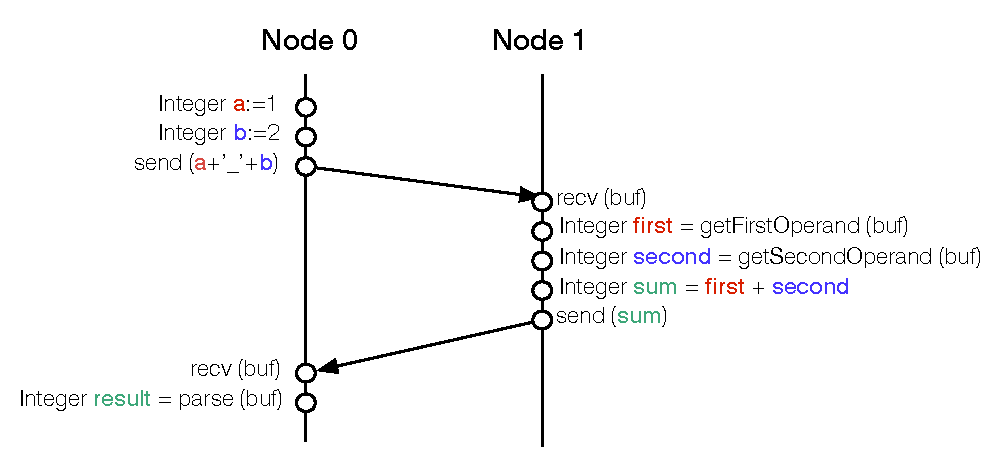
\includegraphics[width=\columnwidth]{sample_code.pdf}
  \caption{Example communication between two nodes in a distributed system}
  \label{fig:sample_code_diag}
\end{figure}

\begin{figure}
\begin{lstlisting}[caption={Sample code for Communication between 2 nodes - Node 0}, label=lst:node0]
    Integer a := 1
    Integer b := 2
    send ( a + '_' + b )
    recv (buf)
    Integer result := parse (buf)
\end{lstlisting}
\end{figure}

\begin{figure}
\begin{lstlisting}[caption={Sample code for Communication between 2 nodes - Node 1}, label=lst:node1]
    recv (buf)
    Integer first := getFirstOperand( buf )
    Integer second := getSecondOperand( buf )
    Integer sum := first + second
    send ( sum )
\end{lstlisting}
\end{figure}

As mentioned earlier, the naive approach for inferring these invariants will be to dump all
state variable values at all program points and feed them to an
invariant detector like Daikon\cite{ernst2007daikon}. But given the
number of program points and huge number of variables in a relatively
large program this approach is not scalable. Moreover, it can result in inferring incorrect invariants that are hold by accident. So we propose two main
optimizations to reduce the number of program point, variable value
combinations.

\subsection{Detecting interesting program points}

Rather than dumping state at all program points we expect the
developer to mark interesting program points using annotations. The
program state will be dumped at only these annotated points. This will
also help to narrow down the focus to points that are identified by
the developer as interesting points without wasting resources
analyzing useless program points. The annotations will be identified
by the parser at the instrumentation phase and re-written to include
statements which will write the values of variable to a file when the
program reaches that point in the runtime. Since there can be multiple points annotated in a program by a
developer, vector clocks will be used to partially order annotation
pairs in the two programs.% This will also help to invalidate
% annotations inserted at irrelevant locations by the developer.

\subsection{Data and Control Flow analysis for Go programs}

Even at interesting program points, variable space that need to be
captured is very large and also we want to filter out irrelevant invariants by only considering variables that affect each other for invariant detection phase. So only the variables that were affected by
the communication with other nodes need to be identified (distributed state variables).  To detect
these variables, some form of data and control flow analysis is required. For example using a backward flow analysis on Listing~\ref{lst:node1} we can say that \texttt{sum} variable at line 4 and line 5 is affected by the \texttt{buf} variable and receive function at line 1. Note that \texttt{sum} variable is part of distributed state of the system, since its value is affected by a receive function and affects a send function, so it is possibly affected and affects variables in other nodes of the system (here it is affected variables \texttt{a} and \texttt{b} and affects \texttt{result} in Node 0). To compute these distributed state variables, we developed a Go program slicer which we explain in the following section.

\subsubsection{Go Program Slicer}

``A program slice consists of the parts of a program that (potentially) affect the values computed at some point of interest"\cite{Tip}. For example figure \ref{Fig:backslice} illustrates an example Go program and its computed backward slice from line 11, the sliced program only contains statements that affect value of variables used at line 11 (i.e. product). To identify variables affected by the communication with other nodes we computed the forward slice from receive message functions and computed backward slice from send message functions and determined the variables assigned in these sliced statements. To compute these forward and backward slices we used the approach first proposed by Ottenstein and Ottenstein \cite{PDG}, which used Program Dependence Graph (PDG) and computed slices by checking the reachability of nodes in this graph. PDG captures both control dependency and data dependency of the program, in fact PDG is computed by combining both Data Dependence Graph and Control Dependence Graph (CDG) of a program. For example figure \ref{fig:expdg} depicts the PDG of example program of figure \ref{Fig:backslice}. Figure \ref{fig:pdg} illustrates our approach to compute PDG. First, we computed the Control Flow Graph (CFG) of the program, then from the reversed CFG we computed the post-dominance tree. The Dominance tree is computed by the algorithm proposed by Lengauer and Tarjan \cite{Dom}. In the next step we computed the CDG from post-dominance tree. To compute Data Dependence Graph, first we computed the reaching definitions by solving dataflow equations\cite{dragonbook} and then used $(Def,Use)$ pair to compute the data dependency between associated statements and form Data Dependence Graph. We combined Data and Control Dependence Graphs to compute the PDG. Having the PDG of the program we checked the reachability of nodes in PDG starting from start node to compute forward and backward slices. For example, In PDG of figure \ref{fig:expdg} thick lines are control dependence edges and thin lines are data dependence edges, starting from \texttt{send(product)} node and going backward shaded nodes are reachable, so the shaded nodes are in backward slice of \texttt{send(product)} statement.


\begin{figure}
\begin{subfigure}[b]{\linewidth}
\centering
 \begin{lstlisting}[]
	recv(n)
	i := 1
	sum := 0
	product := 1
	for i <= n {
		sum := sum + i
		product := product * i
		i := i + 1
	}
	send(sum)
	send(product)
\end{lstlisting}
        \vspace{-2mm}
                \caption{A Go Program}
        \end{subfigure}

\begin{subfigure}[b]{\linewidth}
\centering
\begin{lstlisting}[]
	recv(n)
	i := 1

	product := 1
	for i <= n {
		
		product := product * i
		i := i + 1
	}
	
	send(product) // backward slice from here
\end{lstlisting}
        \vspace{-2mm}
                \caption{Go program backward sliced at line 10}
%                \label{Fig:refactored}
        \end{subfigure}
                        \caption{Backward slice of a Go program \cite{Tip} }
                \label{Fig:backslice}
\end{figure}


\begin{figure}
  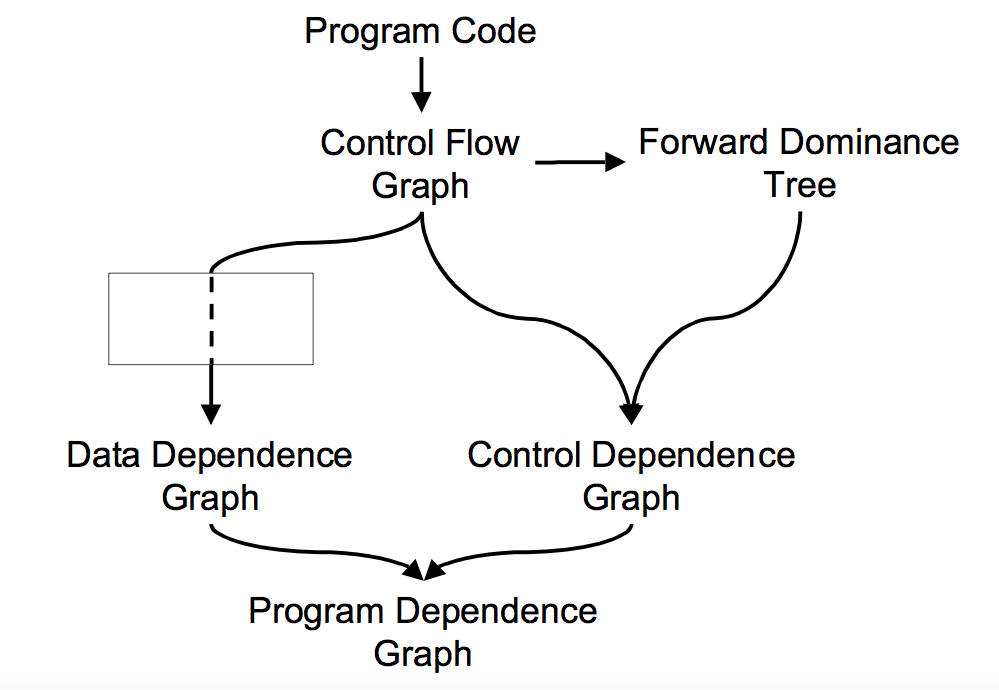
\includegraphics[width=\columnwidth,scale=0.5]{images/PDG-approach.png}
  \caption{Our approach to compute program dependence graph}
  \label{fig:pdg}
\end{figure}


\begin{figure}
  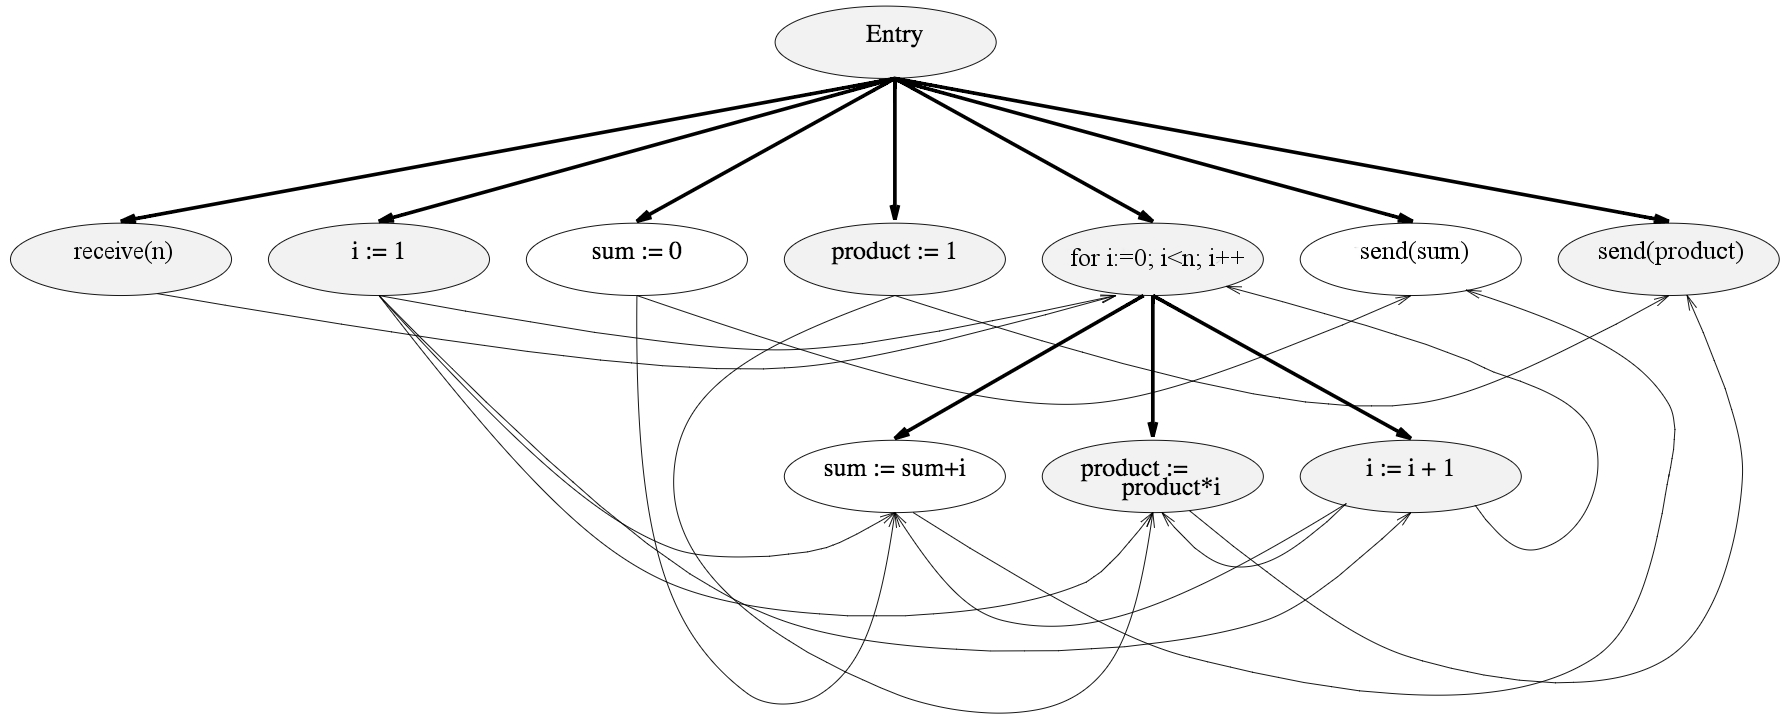
\includegraphics[width=\columnwidth,scale=0.5]{images/pdg.png}
  \caption{Program Dependence Graph of Example Program in Figure \ref{Fig:backslice}}
  \label{fig:expdg}
\end{figure}





%So we are planning to do a dynamic dataflow analysis which consists of following steps:
%\begin{itemize}
%\item Instrumenting variable declarations and assignments at the run time
%\item Collecting execution traces of each of these statements by runnning test suites
%\item Doing a forward flow analysis using the collected traces
%\end{itemize}

%This dynamic analysis approach was chosen because it gives information about the actual execution and therefore is more accurate. And also compared to using a static analysis-based approach, this approach makes it easier to handle Go language-specific constructs like channels which are used share data between goroutines. Only drawback in this approach is, it only examines the paths invoked during execution, unlike static analysis which can be used to reason about all possible execution paths and variable values. To compensate for that we are planning to use a comprehnsive test suite with good test coverage.

% This is a challenging problem in itself because Go language has
% special constructs like channels to share data between goroutines. We
% are planning to do this analysis dynamically by instrumenting variable
% declarations and assignments, and then collecting execution traces of
% each of these statements. We have chosen this approach because it
% gives information about the actual execution and therefore is more
% accurate. For this we are hoping to use static analysis libraries
% available under Go-lang tools\cite{static_golang} which provide
% support for Identifier resolution, Type information, Call graph
% navigation and Channel peers (send $\leftrightarrow$ receive)
% identification.

% Our dynamic dataflow analysis is focused on mainly providing the
% following features. Given a variable, start line and end line it will
% return a set of variables affected by that variable between start line
% and the end line.

% As the next phase of our project, using the above analysis, we hope to
% find out variables affected by receiving messages in interprocess
% communication channels like RPC and TCP/UDP sockets. We will get the
% values of these variables just before another send/receive or end of
% function whichever occurs first. We assume these set of variables at
% the send statement in both (sending and receiving) nodes taken
% together represent global state of the distributed system.

% Given two nodes which are communicating we have two such sets of
% variables representing a particular state. So we will select the
% corresponding variable pairs from send and receive of each node
% mentioned in the previous step and provide as inputs for the Daikon
% invariant detector. This will give us a set of properties that were
% true over the observed executions across 2 nodes. Overall execution
% flow of the analysis is shown in Figure~\ref{fig:go_flow}.

Overall execution flow of the analysis is illustrated in Figure~\ref{fig:go_flow} and works as follows:
\begin{itemize}
\item Developer annotates interesting program points in the Go program which will be used as states for mining invariants.
\item Program Dependence Graph is computed and based on the location of send, receive and developer annotated points, set of variables that contribute to distributed state of the system and thus should be dumped at each point is determined
\item Program is instrumented to dump selected variable values, their type and current vector clock at the annotated program points at run time
\item Based on the vector clock of each log, logs are paired to each other and combined variable values of two logs is fed to the daikon in its specific format.
%For this we are hoping to use static analysis libraries
%available under Go-lang Parse package and tools\cite{static_golang} which provide
%support for Identifier resolution, Type information, Call graph
%navigation and Channel peers (send $\leftrightarrow$ receive)
%identification.
%\item Then as the first step in the analysis phase, this instrumented program is executed using the test suites and program traces are collected.
%\item Forward flow analysis is done on the collected traces
%\item Using the results of the previous step, variables contributing to distributed state is identified.
%\item From the dumped variable values at annotated program points (after multiple executions), only the values of variables chosen in the previous step are selected.
%\item Selected variable values belonging to 2 distinct annotated program points in the 2 nodes are fed to Daikon for inferring invariants.
\end{itemize}


\begin{figure}
  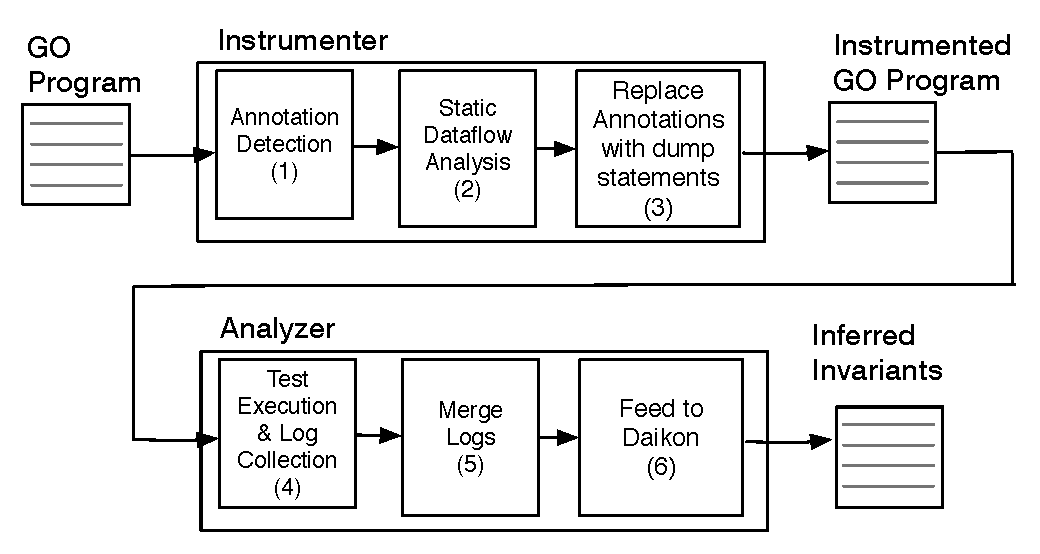
\includegraphics[width=\columnwidth]{go_flow.pdf}
  \caption{Flow of the invariant inference of Go programs}
  \label{fig:go_flow}
\end{figure}

% \section{Timeline}

% Following is the planned milestones and estimated timeline for the project completion.

% \begin{description}
%   \item[2/10:] Proposal Draft Submission
%   \item[3/3:] Proposal Submission
%   \item[3/7:] Finalizing the design, Familirization with required tools (Daikon, Go source analysis tools)
%   \item[3/14:] Implementation - Go program instrumentation to handle annotations and dumping state
%   \item[3/21:] Implementation - Dynamic Forward Analysis for Go programs
%   \item[3/28:] Implementation - Vector clocks integration and end-to-end working analysis
%   \item[4/4:] Evaluation - Inferring invariants in test programs
%   \item[4/7:] Project Presentation
%   \item[4/16:] Project Code and Report Submission
% \end{description}